\section{Problem formulation}
\label{sec:otj:problem}

\begin{figure}[t]
  \begin{centering}
  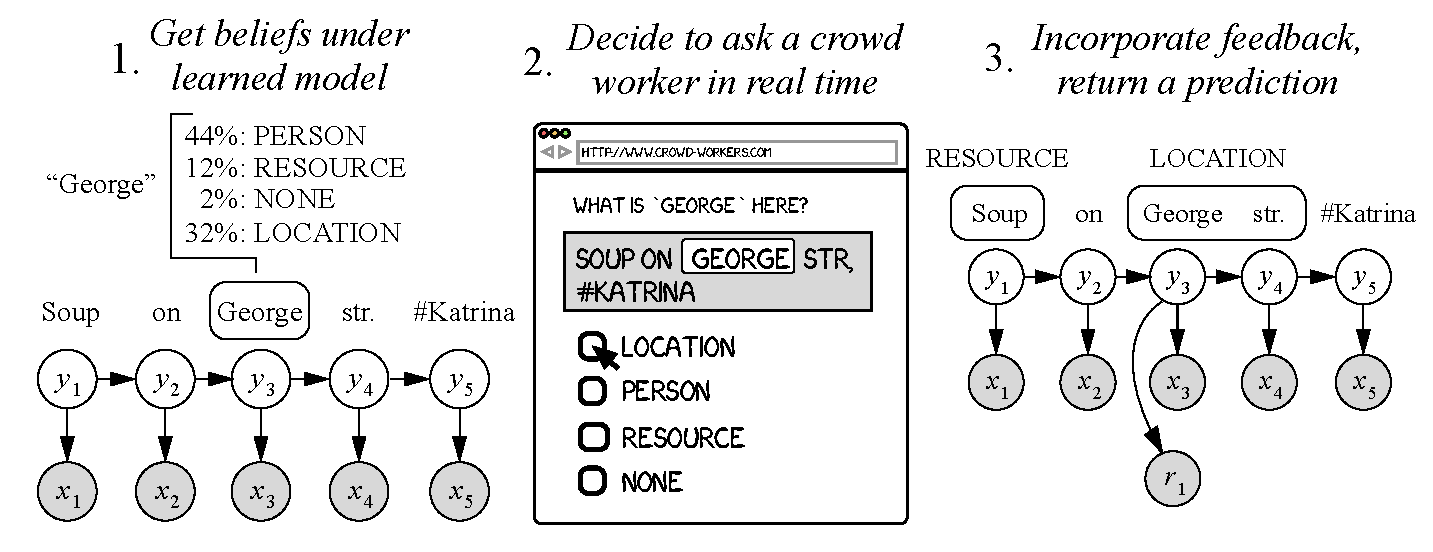
\includegraphics[width=1.0\textwidth]{figures/intro-banner.pdf}
  \end{centering}
  \caption{\label{fig:otj:crf}
    Named entity recognition on tweets in on-the-job learning.
    %(1) The system first runs a
%pre-trained model, discovers that the token ``George'' is ambiguous, and then
%asks a human for a label. The human label is returned in a few seconds,
%incorporated into the model, and the model then decides it has enough
%information to turn in a classification.
}

\end{figure}

% Define structured prediction
Consider a structured prediction problem from input $\bx = (x_1, \dots, x_n)$ to output $\by = (y_1, \dots, y_n)$.
For example, for named-entity recognition (NER) on tweets,
$\bx$ is a sequence of words in the tweet (e.g., \nl{on George str.})
and $\by$ is the corresponding sequence of labels (e.g., \scnone{} \scloc{} \scloc{}).
The full set of labels of \scper{}, \scloc{}, \scres{}, and \scnone{}.

% Basic setting
In the \emph{on-the-job learning} setting, inputs arrive in a stream.
On each input $\bx$,
we make zero or more queries $q_1, q_2, \dots$ on the crowd to obtain labels
(potentially more than once)
for any positions in $\bx$.
The responses $r_1, r_2, \dots$ come back asynchronously,
which are incorporated into our current prediction model $p_\theta$.
\reffig{otj:tree} shows one possible outcome:
We query positions $q_1 = 2$ (\nl{George}) and $q_2=3$ (\nl{str.}).
The first query returns $r_1 = \scloc$,
upon which we make another query on the the same position $q_3 = 3$ (\nl{George}),
and so on.
When we have sufficient confidence about the entire output,
we return the most likely prediction $\hat \by$ under the model.
Each query $q_i$ is issued at time $s_i$ and the response comes back at time $t_i$.
Assume that each query costs $m$ cents.
Our goal is to choose queries to maximize accuracy, minimize latency and cost.

% More intuition / connections
We make several remarks about this setting:
First, we must make a prediction $\hat \by$ on each input $\bx$ in the stream,
unlike in active learning, where we are only interested in the pool or stream of examples
for the purposes of building a good model.
Second, the responses are used to update the prediction model, like in online learning.
This allows the number of queries needed (and thus cost and latency) to decrease over time
without compromising accuracy.
